%\documentclass{article}
%\usepackage[pdftex,active,tightpage]{preview}
%\usepackage{tikz}
%\usepackage{pgfplots}
%\usetikzlibrary{plotmarks}
%\begin{document}
%\begin{preview}
	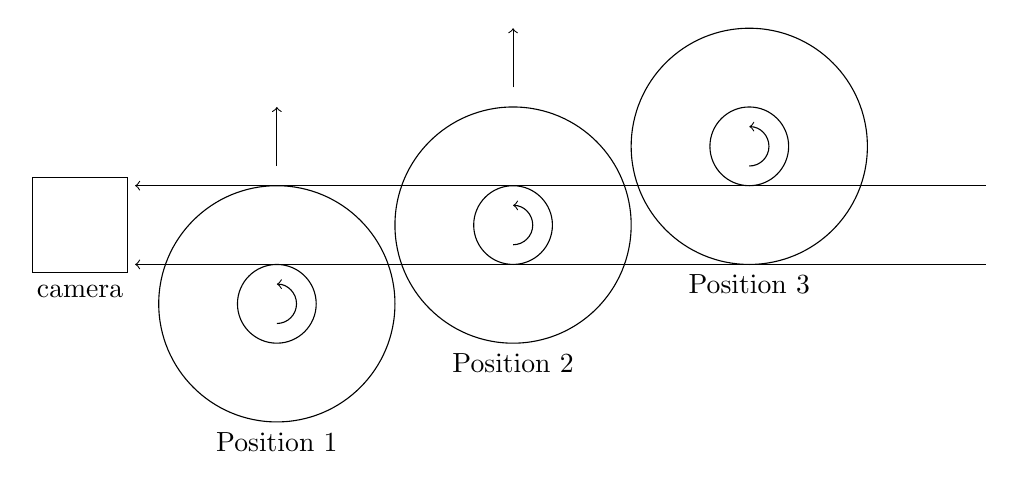
\begin{tikzpicture}[scale=1]
		%drawing grid
%		\draw[color=gray] (0,0) grid (10,1);
		%camera
			\draw (-.1,-.1) rectangle (1.1,1.1);
			\draw (.5,-.35) node {camera};
		% sample positions
			\foreach \x in {1,2,3}{
				\draw     (3*\x,\x-1.5) circle (.5) circle (1.5);			
				\draw[->] (3*\x,\x-1.75) arc (-90:90:.25);
				\draw     (3*\x,-3.25+\x)node {Position \x};
				}
		% movement		
			\foreach \x in {1,2}{				
			    \draw[->]  (3*\x,0.25+\x) -- (3*\x,1+\x);
		% beam
				\draw[<-] (1.2,\x-1) -- (12,\x-1);
				}
	\end{tikzpicture}
%\end{preview}
%\end{document}